% !TEX root = EvoTree-KDD.tex

\section{Related Work}\label{sec:related-work}
%In this section, we briefly review the techniques that are most relevant to our work.
%In general, they can be grouped into two areas: evolutionary topic analysis and visual topic evolution.

\begin{figure*}[t]
  \centering

  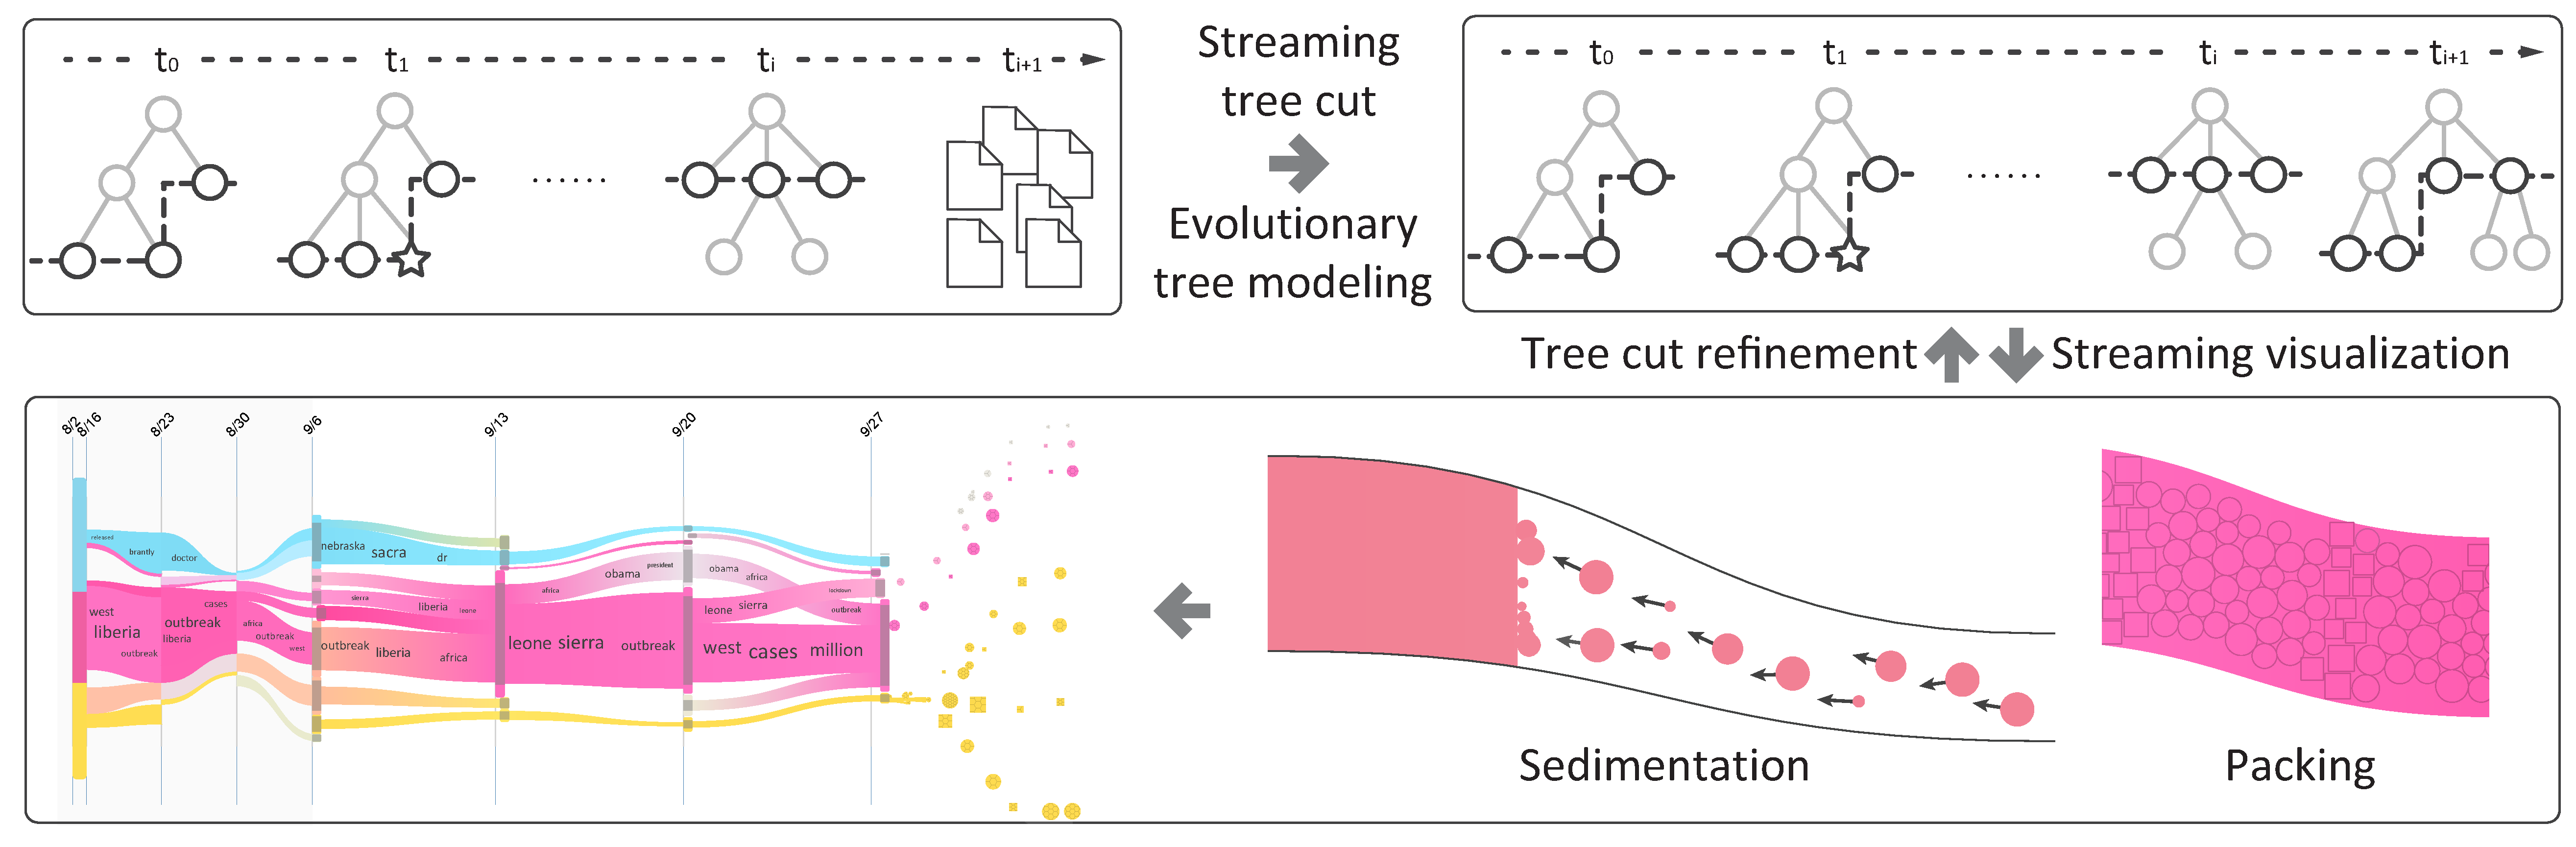
\includegraphics[width=\linewidth]{fig/system}
  \vspace{-5mm}
  \caption{\emph{\normalsize TopicStream} system consists of two modules: streaming tree cut and streaming visualization.}
  \label{fig:overview}
  \vspace{-2mm}
\end{figure*}

\subsection{Evolutionary Topic Analysis}
%Various generative-probabilistic-model-based machine learning algorithms, such as dynamic Latent Dirichlet Allocation (LDA)~\cite{Ahmed2010,blei2006,Blei2012} and hierarchical Dirichlet processes~\cite{Ahmed2008,Xu2008,Xu2008a,Zhang2010}, have been proposed to extract evolving topics from a text stream.
Various generative-probabilistic-model-based machine learning algorithms, such as dynamic Latent Dirichlet Allocation (LDA)~\cite{blei2006} and hierarchical Dirichlet processes~\cite{Ahmed2008,Ahmed2010,Xu2008a,Zhang2010}, have been proposed to extract evolving topics from a text stream.
%To effectively identify a large number of topics from millions of news articles, MemeTracker~\cite{Leskovec2009} was developed.
MemeTracker~\cite{Leskovec2009} was developed to effectively identify phrase-based topics from millions of news articles.
%It provides a coherent representation of the news cycle and  allows users to track the temporal behaviors of memes represented by short phrases.
%\kg{This tool} provides a coherent representation of the news cycle and  allows users to track the temporal \kg{behavior} of memes represented by short phrases.
In many applications, evolving topics may be related to or correspond to one another over time.
%Evolving topics \kg{in many applications can} be related to or correspond \kg{to} one another over time.
The most intuitive relationships are \emph{\normalsize topic correlation}~\cite{wang2007} and \emph{\normalsize common topics}~\cite{wang2009}.
%Recent efforts have also been extended to analyze topic evolution patterns in text data, including topic birth, death, splitting, and merging~\cite{Gao2011}.
Recent efforts have focused on the analysis of topic evolution patterns in text data, including topic birth, death, splitting, and merging~\cite{Gao2011}.
%Although the above-mentioned methods helped users understand a text corpus, none of them focuses on mining and understanding streaming hierarchical topics.
%Although the \kg{aforementioned} methods \kg{help} users understand a text corpus, none of \kg{these} focuses on mining and understanding streaming hierarchical topics.
Although the aforementioned methods help users understand a text corpus, none of them focus on mining and understanding streaming hierarchical topics.

%A previous study has shown that users can better understand and consume information if they are provided with hierarchical topic information over time~\cite{Zhang2009}.
%Some efforts have been exerted recently to mine hierarchical topics and their evolving patterns in temporal datasets efficiently and effectively.
Some efforts have also been exerted recently to mine hierarchical topics and their evolving patterns in temporal datasets.
 %efficiently and effectively.
%The evolutionary hierarchical clustering algorithm~\cite{Chakrabarti2006} aims at generating a sequence of hierarchical clusters.
The evolutionary hierarchical clustering algorithm~\cite{Chakrabarti2006} generates a sequence of hierarchical clusters.
%It aims to cluster data over time.
%The major feature of this algorithm is that clustering at any time fits the current data well.  Furthermore, the clustering does not shift dramatically from one time point to the next when the content is similar.
%The major feature of this algorithm is that clustering \kg{properly} fits current data \kg{at any time}. Furthermore, clustering does not shift dramatically from one time point to the next when \kg{contents} are similar.
The major feature of this algorithm is that clustering properly fits current data at any time (fitness). Furthermore, clustering does not shift dramatically from one time step to the next when content is similar (smoothness).
However, this algorithm can only generate evolving binary trees.
To tackle this issue, Wang et al.~\cite{Wang2013}
% proposed an evolutionary multi-branch tree clustering method.
%In this method, tree construction is formulated as an online posterior estimation problem that considers both the likelihood of the current tree and the conditional prior given the previous tree.
%In this method, tree construction \kg{was} formulated as an online posterior estimation problem that \kg{considered} both the likelihood of the current tree and the conditional prior given the previous tree.
formulated the multi-branch tree construction problem as  a Bayesian online filtering process.
 %that \dc{considers} both the fitness of the current tree and the conditional prior given the previous tree.
%Compared with the method proposed in~\cite{Wang2013}, our method addresses the problem of how to better understand and analyze a sequence of evolutionary multi-branch topic trees.
%\kg{Unlike} the method proposed in~\cite{Wang2013}, our method addresses the problem of \kg{better understanding} and analyze a sequence of evolutionary multi-branch topic trees.
Unlike the method proposed in~\cite{Wang2013}, our method addresses the problem of better understanding and analyzing a sequence of evolutionary multi-branch topic trees.
%Technically, we first learn a set of evolutionary tree cuts from the topic trees based on the user-selected focus nodes.
We first learn a set of evolutionary tree cuts from the topic trees based on the user-selected focus nodes.
%Then we design a time-based interactive visualization to allow users to examine hierarchical topic evolution from multiple perspectives.
Then we design a sedimentation-based interactive visualization to reveal hierarchical topic evolution from multiple perspectives.

%introduce two constraints, triples and fans, into the model to guarantee high smoothness between topic trees. In addition, we also choose the Bayesian rose tree~\cite{Blundell2010} as our base representation to discover multi-branch structures in text data instead of binary tree structures.\looseness=-1

\subsection{Visual Topic and Event Evolution}

The visual analysis of evolving topics in text corpora has been widely studied in recent years~\cite{cui2011,Havre2002,Liu2014survey,Sun2013survey}.
Many methods utilize a river metaphor (a stacked graph) to convey evolving topics over time.
For example, ThemeRiver~\cite{Havre2002} visually depicts how keyword strengths change over time in a text corpus through a river metaphor.
A layer represents a topic in this metaphor.
%The varying width of a layer represents the strength change over time.
The varying width of a layer represents \dc{strength} change over time.
%TIARA~\cite{Liu2009,Liu2012} tightly integrates interactive visualization with topic analysis techniques to help users better understand a document collection.
TIARA~\cite{Liu2009,Liu2012}
%tightly integrates interactive visualization with topic analysis techniques to help users \kg{understand} a document collection.
%In particular, it
%employs the LDA model~\cite{blei2003} to analyze a large text corpus and then
employs an enhanced stacked graph to illustrate how topics evolve over time.
%To model the relationships between evolving topics,
%ParallelTopics~\cite{Dou2011} utilizes ThemeRiver to illustrate topic evolution over time and parallel coordinate plots to reveal the probabilistic distribution of a document on different topics.
ParallelTopics~\cite{Dou2011} utilizes ThemeRiver to illustrate topic evolution over time and parallel coordinate plots to reveal the probabilistic distribution of a document on different topics.
TextFlow~\cite{cui2011} was developed to help analysts visually analyze topic merging and splitting relationships and track their evolution over time.
A visual analysis system was designed by Xu et al.~\cite{Xu2013} to allow analysts to interactively explore and understand the dynamic competition relationships among topics.
% and the influence of opinion leaders.
Recently, Sun et al.~\cite{GSun2014a} extended this work to study both the cooperation and competition relationships among topics.\looseness=-1
%TextFlow~\cite{cui2011} was developed to help analysts visually analyze \kg{the} merging and splitting relationships \kg{of topics} and track their evolution over time.

Several visualization techniques have been proposed recently to help users analyze temporal events and their evolving patterns~\cite{Dou2012,krstajic2013,Luo2012}.
EventRiver~\cite{Luo2012} assumes that clusters of news articles with similar content are adjacent in time and can be mapped to events.
%Thus, this method automatically detects important events and visually presents their impact over time.
Thus, this method automatically detects important events and visually presents their impact over time.
LifeFlow~\cite{Wongsuphasawat2011} and Outflow~\cite{Wongsuphasawat2012} help users explore temporal event sequences.
%\dup{They aggregate multiple event sequences into a tree and a directed acyclic graph, respectively.}
%Timeline visualization is then employed to display the aggregated event sequences from multiple aspects.
%Timeline visualization is then employed to display aggregated event sequences from multiple aspects.\looseness=-1

%In addition, several researchers have proposed word-based approaches to illustrate the content evolution of text data.
%By leveraging the advantages of both parallel coordinates and traditional tag clouds, Collins et al.~\cite{Collins2009} developed Parallel Tag Clouds to support faceted browsing of text corpora.
%Tightly integrating tag clouds with sparklines, SparkClouds~\cite{Lee2010} aimed to visually explain the temporal trend inside tag clouds. To achieve this, it tightly integrated tag clouds with sparklines.

%The above-mentioned approaches focus on the visual exploration of evolving topics/events with flat structures.
%The \kg{aforementioned} approaches focus on visual the visual exploration of evolving topics/events with flat structures.
The aforementioned approaches focus on the visual exploration of evolving topics/events with flat structures.
%Our work attempts to support the visual analysis of evolving hierarchical topics over time.
%\kg{By contrast,} our work attempts to support the visual analysis of evolving hierarchical topics over time.
By contrast, our method attempts to support the visual analysis of evolving hierarchical topics over time.

%HierarchicalTopics~\cite{Dou2013} hierarchically organizes the extracted topics by the BRT model~\cite{Blundell2010,Liu2012} and thus can represent a large number of topics without being cluttered.
HierarchicalTopics~\cite{Dou2013} hierarchically organizes topics using the BRT model~\cite{Blundell2010,Liu2012a}, which can then represent a large number of topics without being cluttered.
%However, this method utilizes one static tree to organize all the topics and cannot illustrate the splitting/merging relationships among topics.
However, this method utilizes one static tree to organize all topics and cannot illustrate splitting/merging relationships among topics.\looseness=-1

To solve this problem, Cui et al.~\cite{cui2014} developed \emph{\normalsize RoseRiver} to progressively explore and analyze the complex evolution patterns of hierarchical topics.
%Cui et al.~\cite{cui2014} made an initial effort to help users progressively explore and analyze the complex evolution patterns of hierarchical topics \kg{and solve the aforementioned problem}.
%This visual analytics system introduces the concept of evolutionary tree cuts and help analysts better understand large document collection with time-stamps.
This system introduces the concept of evolutionary tree cuts to help better understand large document collection with time-stamps.
%However, it fails to provide a mechanism analyze the streaming data because a global evolutionary tree cut algorithm is employed.
However, it fails to provide a mechanism to analyze streaming data because a global tree cut algorithm is employed.
%In addition, the authors used the degree-of-interest-based heuristic rule to derive the key tree cut, which may not be the optimal solution.
In addition, the authors used the DOI-based heuristic rule to derive the key tree cut, which may not be the optimal solution.

%Compared with this method, we employ a posterior probability to derive the optimal tree cut for a selected tree (seed tree cut).
Unlike the preceding method, we employ a-posterior-probability-based method to estimate the fitness of the tree cut.
%In order to help analysts understand the topics of interest in the incoming data, we formulate the derivation of the tree cut in incoming data as the HMM.
We then formulate the derivation of the tree cut in incoming data as a DBN.
% to help analysts understand the topics of interest in incoming data.
%The quantitative evaluation in Sec.~\ref{sec:evaluation} shows that the posterior probability method performs better than the DOI-based method in~\cite{cui2014} for deriving the seed tree cut.
%The quantitative evaluation in Sec.~\ref{sec:evaluation} shows that the posterior probability method performs better than the DOI-based method in~\cite{cui2014} \kg{in} deriving the seed tree cut.
The quantitative evaluation in Sec.~\ref{sec:quantitativeevaluation} shows that the posterior-probability-based method performs better than the DOI-based method in~\cite{cui2014} to fit the focus nodes and topic trees.
%The the performance of the HMM-based streaming evolutionary tree cut algorithm is comparable to that of the global evolutionary tree cut algorithm proposed in~\cite{cui2014}.
The performance of the DBN-based streaming tree cut algorithm is comparable with that of the global tree cut algorithm proposed in~\cite{cui2014}.
%This demonstrates the effectiveness of the proposed mining algorithms in handling the new coming datas in text streams.
%\kg{These observations} demonstrate the effectiveness of the proposed mining algorithms in handling \kg{incoming} data in text streams.
These observations demonstrate the effectiveness of the proposed mining algorithms at handling incoming data in text streams.
%An improved visual sedimentation metaphor~{Huron2013visual} is adopted is visually illustrate how the new coming text streams are aggregating into the existing topic archive.
%An improved visual sedimentation metaphor~\cite{Huron2013visual} is adopted to visually illustrate how \kg{incoming} text streams \kg{aggregate into} existing topics.
An improved visual sedimentation metaphor~\cite{Huron2013visual} has been adopted to visually illustrate how incoming text streams aggregate into existing topics.

%\pei{By saying this, do we mean there are some other methods "to support visual analysis of evolving hierarchical topics over time"?  If so, we have to review those methods.  If not, we need to move the word "among".}

%Inspired by XKCD's movie narrative charts~\cite{RMunroe}, a storyline visualization has been developed to illustrate the temporal interactions between characters in a story.
%Ogawa and Ma~\cite{Ogawa2010} developed a set of heuristic rules to quickly generate a storyline layout.
%Although this method can generate a storyline layout in real time, it may generate a layout with many line crossings and wiggles.
%To overcome this limitation, Tanahashi and Ma~\cite{YTanahashi2012a} formulated the storyline layout as an optimization problem.
%They leveraged spatial information to convey hierarchical relationships among characters.
%However, the hierarchical information was not considered in the layout algorithm but was added in the post-processing step.
%As a result, it cannot leverage the location hierarchy to handle a large number of character lines.
%Different from this method, our method aims to generate a set of evolving topic trees and use them to organize a large number of topics over time.
%To better present evolving hierarchical topics on limited screen real estate, an evolving tree cut algorithm is proposed to extract an appropriate number of topics for each tree, based on the user selected focus node(s).


